\documentclass[10pt,journal]{IEEEtran}

\usepackage[T1]{fontenc}
\usepackage{lmodern}
\usepackage{amsmath,amssymb,bm}
\usepackage{booktabs,array,multirow}
\usepackage{graphicx}
\usepackage{xcolor}
\usepackage{pgfplots}
\usepackage{microtype}
\usepackage{listings}
\usepackage{url}
\usepackage[hidelinks]{hyperref}

\pgfplotsset{compat=1.18}
\definecolor{reportblue}{HTML}{2A6FBB}
\definecolor{reportorange}{HTML}{E67E22}
\definecolor{reportgray}{HTML}{4B5563}
\definecolor{reportlight}{HTML}{EEF2F7}
\definecolor{reportred}{HTML}{B42318}

\hypersetup{
  pdftitle={Reproducing a GPU-Based sGS-HPR Solver for Large-Scale Multi-Period DC Optimal Power Flow},
  pdfauthor={Thomas DiGregorio},
  pdfsubject={Stage 9 final structural reproduction report},
  pdfkeywords={DCOPF, sGS-HPR, GPU, DGX Spark, reproducibility}
}

\newcommand{\classresult}{\textbf{D -- Structural Reproduction}}
\newcommand{\sgshpr}{sGS-HPR}
\newcommand{\R}{\mathbb{R}}
\newcommand{\norm}[1]{\left\lVert #1\right\rVert}
\newcommand{\pathcode}[1]{\begingroup\urlstyle{tt}\url{#1}\endgroup}

\lstset{
  basicstyle=\ttfamily\scriptsize,
  breaklines=true,
  columns=fullflexible,
  frame=single,
  rulecolor=\color{reportlight},
  showstringspaces=false
}

\title{Reproducing a GPU-Based sGS-HPR Solver for Large-Scale Multi-Period DC Optimal Power Flow:\\
An Evidence-Bounded Structural Reproduction on NVIDIA DGX Spark}

\author{Thomas~DiGregorio%
\thanks{Independent reproduction study completed August 5, 2026. Source,
machine-readable evidence, and regeneration commands are maintained in the
sGS-HPR-DC-SCOPF repository.}}

\begin{document}
\maketitle

\begin{abstract}
This work reproduces the mathematical and computational structure of the
symmetric Gauss--Seidel Halpern-accelerated proximal-reflection (\sgshpr{})
method reported by Wang \emph{et al.} for large-scale multi-period DC optimal
power flow (DCOPF). We reconstruct the canonical linear program, implement the
paper-order dual updates, independently verify the KKT and stopping maps,
correct a sign inconsistency in the printed structural equality inverse, build
an FP64 CPU oracle, and port the validated path to an NVIDIA DGX Spark. The GPU
path proves low-level cuSPARSE CSR ALG2 selection, resident iterative state,
and trajectory parity with the CPU implementation.

Public MATPOWER networks and deterministic renewable/storage policies are used
to reconstruct all 18 rows of the paper's main benchmark table. All 18 row and
variable dimensions match the publication, but none of the sparse nonzero
counts match because the authors' modified instances and construction pipeline
are unavailable. Six Stage 7 rows pass HiGHS, CPU FP64, GPU FP64, numerical,
physical, provenance, and repeated-timing gates. Stage 8 adds four fully
passing large rows. On \texttt{case9241pegase:T6}, HiGHS and GPU FP64 pass,
while the required CPU FP64 correctness solve exceeds the frozen 3,600-second
deadline. The final three requested rows are resolved without allocation: T16
exceeds both live unified-memory budgets, and T24/T32 exceed signed-int32 CSR
planning capacity. We therefore classify the result as \classresult{}, not an
exact, near-exact, or controlled performance reproduction.
\end{abstract}

\begin{IEEEkeywords}
DC optimal power flow, Halpern iteration, proximal reflection, symmetric
Gauss--Seidel decomposition, GPU sparse linear algebra, reproducibility, DGX
Spark.
\end{IEEEkeywords}

\section{Introduction}

The central question of this reproduction is not merely whether a GPU program
can solve a related DCOPF. It is whether the mathematical route in
\cite{wang2026} can be rebuilt, checked against independent oracles, ported
without changing the algorithmic path, and scaled transparently enough to
distinguish reproduction from reconstruction or resource limitation.

The answer has three parts. First, the canonical LP, Algorithm 2 update order,
KKT map, stopping tests, structural equality solve, CPU oracle, and resident
FP64 GPU path were independently checked. Second, the authors' numerical
instances were not reproduced: public-network reconstructions match every
published row and variable dimension but differ in every sparse nonzero count.
Third, the full large-scale acceptance campaign did not pass. Four Stage 8
rows passed; a fifth failed when its required CPU correctness track timed out;
later rows were safely stopped by memory and index guards.

This distinction is critical. An independent checker PASS establishes that a
protocol was followed and evidence preserved. It cannot convert a failed
scientific acceptance gate into a successful result. The final classification
is therefore \classresult{}.

\subsection{Contributions}

This report contributes:
\begin{itemize}
  \item a line-by-line mathematical specification of the canonical DCOPF and
  \sgshpr{} updates;
  \item independent projection, residual, direct-solve, spectral, physical,
  and CPU/GPU trajectory checks;
  \item a documented correction to the paper's rank-one inverse;
  \item a resident FP64 DGX implementation with observed CSR ALG2 selection
  and transfer auditing;
  \item an 18-row structural ledger and an 11-row allocated benchmark record;
  \item fail-closed unified-memory and signed-int32 resource evidence; and
  \item a machine-readable index, deterministic table generator, command
  inventory, and reproducibility checklist.
\end{itemize}

The optional N-1 extension is outside scope and remains locked.

\section{Source Paper and Reproduction Boundary}

The reproduced source is \emph{An Efficient GPU-based Halpern Accelerating
Algorithm for Large-scale DC Optimal Power Flow} by Wang \emph{et al.}
\cite{wang2026}. The supplied 17-page PDF has SHA-256
\begin{center}
\scriptsize\url{7e9791646401e11bfddf9ebed6bd94491ed0b592744581edd851ddbf5e20dba4}.
\end{center}
The paper writes a multi-period base-case DCOPF as a box-constrained LP,
applies HPR to its dual, and exploits the equality/inequality partition with a
symmetric Gauss--Seidel sweep. The equality block admits a diagonal plus
low-rank solution; the inequality multiplier update is a projected spectral
step. The authors prove an $O(1/k)$ non-ergodic KKT residual rate and summarize
large-system complexity as $O(N_Ln/\epsilon)$.

The paper reports an A100-SXM4-80GB, CUDA 12.3, CSR storage, and cuSPARSE CSR
ALG2. Gurobi 12.0 is timed on a separate Intel i9-14900HX workstation. The
publication calls the problem security-constrained, but the displayed model
contains no outage or contingency index. This work therefore treats the
printed formulation as base-case multi-period DCOPF. An N-1 SCOPF model would
be new research rather than part of this reproduction.

\section{Mathematical Formulation}

\subsection{Canonical primal and dual}

The implementation contract is the paper's canonical linear program
\begin{equation}
\begin{aligned}
\min_{x\in\R^n}\quad & c^{\mathsf T}x,\\
\text{s.t.}\quad & A_1x=b_1,\\
& A_2x\ge b_2,\\
& \ell\le x\le u,
\end{aligned}
\label{eq:primal}
\end{equation}
where $A=[A_1;A_2]$, $b=[b_1;b_2]$, and $C=[\ell,u]$. With
$D=\R^{m_1}\times\R_+^{m_2}$, its dual is
\begin{equation}
\begin{aligned}
\min_{y,z}\quad &-b^{\mathsf T}y+\delta_D(y)+\delta_C^*(-z),\\
\text{s.t.}\quad &A^{\mathsf T}y+z=c.
\end{aligned}
\label{eq:dual}
\end{equation}
Equality multipliers are free and inequality multipliers are nonnegative. The
canonical inequality direction is always $A_2x\ge b_2$.

The reconstructed decision order is
\begin{equation}
x=(p_G,p_{RG},p_{ESS}^{dc},p_{ESS}^{ch},r^u,r^d).
\end{equation}
For $T$ periods, $N_L$ constrained lines, $N_G$ conventional generators,
$N_{RG}$ renewable generators, and $N_{ESS}$ storage devices, the
table-consistent dimensions are
\begin{align}
n &= T(3N_G+N_{RG}+2N_{ESS}),\\
m_1 &= T+N_{ESS},\\
m_2 &= 2TN_L+(4T-2)N_G+2TN_{ESS}+2T.
\end{align}
Power balance and terminal storage energy form $A_1$. Split branch-flow,
headroom/footroom, reserve, ramping, and storage-energy inequalities form
$A_2$. Remaining device limits form the box $C$.

\subsection{KKT and stopping maps}

The full KKT residual is
\begin{equation}
\mathcal{R}(y,z,x)=
\begin{pmatrix}
y-\Pi_D(y-Ax+b)\\
x-\Pi_C(x-z)\\
c-A^{\mathsf T}y-z
\end{pmatrix}.
\label{eq:kkt}
\end{equation}
The paper's stopping rule separately normalizes primal feasibility, box
normal-cone consistency, and stationarity. In particular, its first stopping
block is not the full first block of \eqref{eq:kkt}. Every accepted candidate
must satisfy the three normalized blocks at $5\times10^{-5}$, raw KKT at
$10^{-2}$, original-space physical violations at $10^{-2}$ MW/MWh, and scaled
objective gap to HiGHS at $2\times10^{-4}$.

\section{Implemented sGS-HPR Algorithm}

For $w=(y_1,y_2,z,x)$, the FP64 implementation follows the printed order.
First, the $z$ proximal update and primal multiplier update collapse to
\begin{equation}
\bar x^{k+1}=\Pi_C\left[x^k+\sigma(A^{\mathsf T}y^k-c)\right].
\label{eq:xproj}
\end{equation}
Next, the first equality solve produces $\bar y_1^{k+1/2}$ using $y_2^k$.
The inequality multiplier is then projected as
\begin{equation}
\bar y_2^{k+1}=\Pi_{\R_+^{m_2}}
\left[y_2^k+\lambda^{-1}(b_2/\sigma-A_2R_y)\right],
\label{eq:y2}
\end{equation}
where $\lambda$ safely bounds $\lVert A_2\rVert_2^2$. A second equality solve
produces $\bar y_1^{k+1}$ using the new $\bar y_2^{k+1}$. Both equality sweeps
are required. Finally,
\begin{align}
\widehat w^{k+1}&=2\bar w^{k+1}-w^k,\\
w^{k+1}&=\frac{1}{k+2}w^0+\frac{k+1}{k+2}\widehat w^{k+1}.
\label{eq:halpern}
\end{align}
The anchor $w^0$ is fixed.

Production preprocessing uses ten reversible Ruiz passes, one simultaneous
Pock--Chambolle diagonal step with $\alpha=1$, and complete-vector $b$/$c$
normalization. The manuscript does not publish exact adaptive-penalty and
restart code. Published HPR-LP rules are therefore transferred at the
paper's 100-iteration cadence and explicitly labeled a sourced reconstruction.

\section{Derivation and Implementation Verification}

\subsection{Projection, residual, and physical oracles}

Analytic toy LPs verify box projection, nonnegative multiplier projection, the
combined $z$/$x$ identity, \eqref{eq:kkt}, and the separate stopping blocks.
Independent SciPy HiGHS solves establish objective and multiplier-sign
references. PTDF branch flows are checked against an independent angle solve;
transformer phase shifts are retained as affine offsets. Public base-network
and synthetic storage fixtures remain separate.

\subsection{Structural equality solve and manuscript correction}

For the explicit equality matrix, $A_1A_1^{\mathsf T}$ has diagonal blocks
with rank-one coupling. Eliminating the storage block produces
\begin{equation}
(D_1-\alpha\bm{1}\bm{1}^{\mathsf T})y_{11}=\widetilde R_{11}.
\end{equation}
The manuscript prints the Woodbury sign pattern for a plus rank-one update.
The direct linear-system oracle rejects it. The implementation uses
\begin{equation}
(D_1-\alpha uu^{\mathsf T})^{-1}=D_1^{-1}+
\frac{D_1^{-1}uu^{\mathsf T}D_1^{-1}}
{\alpha^{-1}-u^{\mathsf T}D_1^{-1}u},
\label{eq:woodbury}
\end{equation}
which matches Cholesky in FP64. Stage 4's checker passed 20/20 checks. This is
a documented correction, not a hidden algorithm change.

Dense eigendecomposition is the small-case authority for the proximal
spectral value. Sparse \texttt{eigsh} and seeded power iteration cross-check
it before a positive safety margin is applied. CPU/GPU comparisons test
intermediate trajectories, not only final objectives.

\section{CPU and GPU Implementations}

\subsection{CPU oracle}

The CPU implementation uses SciPy sparse operators, FP64 state, explicit
projections, the paper update order, and both direct and paper-structural
equality backends. All candidates are recovered to original coordinates before
KKT, objective, and power-system checks. It supplies fixed-horizon trajectories
and an independent residual path for GPU validation.

CPU work on the DGX is necessary even in a GPU study: model construction,
reference validation, policy bookkeeping, and an independent oracle cannot be
inferred from GPU success. Stage 8 also preregistered CPU FP64 as a required
track. Consequently, the T6 CPU timeout is a Stage 8 failure even though its
GPU candidate passed. A later user-authorized continuation skipped CPU for
sequences 6--8 without revising the original evidence or contract.

\subsection{Resident FP64 GPU path}

The GPU path uses CuPy arrays and CSR matrices in FP64. $A_1$, $A_2$, their
transposes, scaling vectors, state, and reusable workspaces remain resident. A
phase-labeled transfer ledger permits preparation, scalar diagnostics, policy
checks, and final recovery while rejecting unexpected full-state copies inside
the loop.

Kernel selection is observed, not inferred. A low-level descriptor records
\texttt{CUSPARSE\_SPMV\_CSR\_ALG2} (enum 3 with pinned CuPy 14.1.1), and a probe
verifies normal and transpose products. The largest Stage 6 CPU/GPU sparse
operator error is $2.22045\times10^{-16}$. Full FP64 policy objectives agree
to approximately $1.82\times10^{-11}$ absolute. FP32 is non-gating: it is
finite but misses the frozen FP64 trajectory tolerance and is not represented
as equivalent.

\section{Environment}

\begin{table*}[t]
\caption{Principal reproduction and paper environments.}
\label{tab:environment}
\centering
\small
\begin{tabular}{@{}p{0.20\textwidth}p{0.36\textwidth}p{0.34\textwidth}@{}}
\toprule
Item & Reproduction & Paper \\
\midrule
GPU & NVIDIA GB10, integrated, compute capability 12.1 & NVIDIA A100-SXM4-80GB \\
Memory & 130,663,165,952 bytes (121.69 GiB) unified/global & 80 GB GPU memory \\
Host / OS & Linux/aarch64; Ubuntu 24.04.4; kernel 6.17.0-1029-nvidia & GPU host/OS not specified \\
Python stack & Python 3.12.3; NumPy 2.3.5; SciPy 1.16.3; CuPy 14.1.1 & not specified \\
CUDA & driver API 13.0; runtime API 13.2 & CUDA 12.3 \\
Sparse representation & CSR; signed-int32 indices; FP64 gating path & CSR; index width and precision unstated \\
Gurobi & unavailable and optional locally & v12.0, separate i9-14900HX, 96 GB host \\
\bottomrule
\end{tabular}
\end{table*}

Table~\ref{tab:environment} precludes an exact timing comparison even before
instance differences are considered. The accepted evidence was generated from
clean detached worktrees with executed-source manifests and package pins.

\section{Validation Results}

\begin{table}[t]
\caption{Frozen gates and largest accepted observations.}
\label{tab:gates}
\centering
\scriptsize
\begin{tabular}{@{}lrrc@{}}
\toprule
Gate & Threshold & Maximum & Result \\
\midrule
Normalized primal & $5\mathrm{e}{-5}$ & $2.017\mathrm{e}{-8}$ & Pass \\
Normalized stationarity & $5\mathrm{e}{-5}$ & $9.659\mathrm{e}{-6}$ & Pass \\
Normalized box & $5\mathrm{e}{-5}$ & $8.831\mathrm{e}{-13}$ & Pass \\
Raw KKT & $0.01$ & $0.009635$ & Pass \\
Physical violation & $0.01$ & $0.006311$ & Pass \\
Objective gap & $2\mathrm{e}{-4}$ & $4.285\mathrm{e}{-8}$ & Pass \\
Per-solve deadline & $3600$ s & $3600.093$ s & T6 CPU fail \\
\bottomrule
\end{tabular}
\end{table}

The maxima in Table~\ref{tab:gates} cover completed Stage 7--8 candidates.
The T6 CPU attempt produced no accepted candidate and is represented only by
its timeout.

\begin{table}[t]
\caption{Independent evidence checks versus scientific decisions.}
\label{tab:checks}
\centering
\scriptsize
\begin{tabular}{@{}lccc@{}}
\toprule
Scope & Decision & Checks & Interpretation \\
\midrule
Stages 0--7 & Pass & 120/120 & accepted chain \\
Stage 8 strict & \textbf{Fail} & 12/12 & T6 CPU timeout \\
Stage 8 continuation & resource-limited & 13/13 & no allocation \\
\bottomrule
\end{tabular}
\end{table}

The checker/decision separation in Table~\ref{tab:checks} prevents protocol
integrity from being misread as numerical acceptance.

\section{Benchmark Evidence}

\begin{table*}[t]
\caption{Allocated Stage 7--8 reconstructions. Times are five-repeat local
solver-core medians after correctness and warm-up. A dash denotes no accepted
measurement.}
\label{tab:benchmarks}
\centering
\scriptsize
\setlength{\tabcolsep}{3.6pt}
\begin{tabular}{@{}clrrrrrrl@{}}
\toprule
Stage & Reconstruction & $m$ & $n$ & nnz$(A)$ & HiGHS (s) & CPU (s) & GPU (s) & Result \\
\midrule
7 & case1354 T4  & 20,192  & 4,208   & 4,799,808   & 1.463   & 13.190   & 1.013   & Pass \\
7 & case1354 T16 & 82,124  & 16,832  & 19,228,464  & 7.265   & 47.399   & 2.924   & Pass \\
7 & case1354 T48 & 247,276 & 50,496  & 57,896,368  & 32.095  & 153.046  & 9.481   & Pass \\
7 & case1354 T96 & 495,004 & 100,992 & 116,420,464 & 101.242 & 336.657  & 21.084  & Pass \\
7 & case2868 T4  & 40,163  & 9,488   & 19,073,056  & 5.366   & 60.350   & 3.939   & Pass \\
7 & case2868 T16 & 163,823 & 37,952  & 76,354,336  & 22.138  & 250.601  & 15.408  & Pass \\
8 & case2868 T48 & 493,583 & 113,856 & 229,507,104 & 76.239  & 804.863  & 49.968  & Pass \\
8 & case2868 T64 & 658,463 & 151,808 & 306,303,136 & 108.232 & 1,078.892& 68.383  & Pass \\
8 & case2868 T96 & 988,223 & 227,712 & 460,334,496 & 163.593 & 1,621.905& 105.022 & Pass \\
8 & case9241 T4  & 152,774 & 24,700  & 342,863,272 & 142.479 & 3,087.218& 193.632 & Pass \\
8 & case9241 T6  & 230,376 & 37,050  & 514,308,838 & 963.957 & --       & 357.544 & \textbf{Fail} \\
\bottomrule
\end{tabular}
\end{table*}

The GPU completed and validated all 11 allocated rows in
Table~\ref{tab:benchmarks}; the CPU completed 10. Stage 8's fully passing
prefix is four because all required tracks had to pass.

\begin{figure*}[t]
\centering
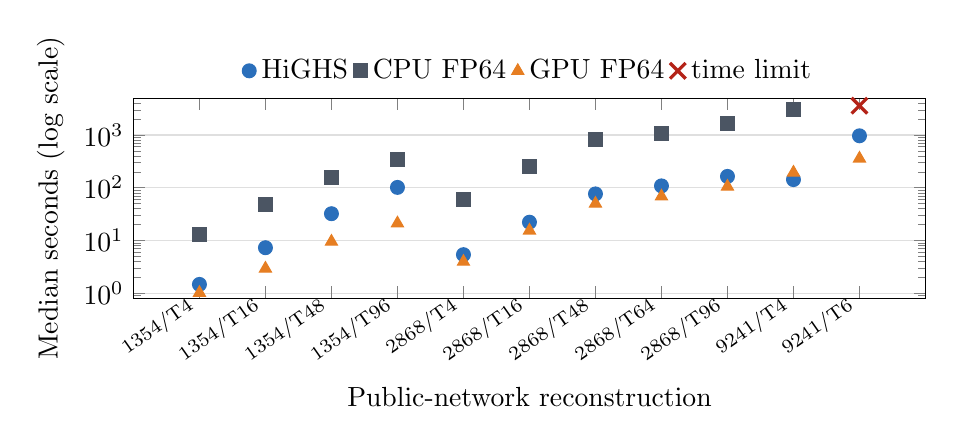
\begin{tikzpicture}
\begin{axis}[
  width=0.96\textwidth,
  height=0.34\textwidth,
  ymode=log,
  ymin=0.8,
  ymax=5000,
  ylabel={Median seconds (log scale)},
  xlabel={Public-network reconstruction},
  xtick={0,...,10},
  xticklabels={1354/T4,1354/T16,1354/T48,1354/T96,2868/T4,2868/T16,2868/T48,2868/T64,2868/T96,9241/T4,9241/T6},
  xticklabel style={rotate=35,anchor=east,font=\scriptsize},
  ymajorgrids=true,
  grid style={draw=gray!25},
  legend style={at={(0.5,1.02)},anchor=south,legend columns=4,draw=none},
  mark size=2.5pt,
]
\addplot[only marks,mark=*,reportblue,fill=reportblue] coordinates {
  (0,1.463376) (1,7.265354) (2,32.095478) (3,101.242296)
  (4,5.366418) (5,22.138002) (6,76.238645) (7,108.232479)
  (8,163.592526) (9,142.478889) (10,963.956952)};
\addlegendentry{HiGHS}
\addplot[only marks,mark=square*,reportgray,fill=reportgray] coordinates {
  (0,13.190169) (1,47.398903) (2,153.046368) (3,336.657478)
  (4,60.349654) (5,250.601316) (6,804.863493) (7,1078.891699)
  (8,1621.905045) (9,3087.217721)};
\addlegendentry{CPU FP64}
\addplot[only marks,mark=triangle*,reportorange,fill=reportorange] coordinates {
  (0,1.013252) (1,2.924268) (2,9.480950) (3,21.084461)
  (4,3.938934) (5,15.408042) (6,49.968351) (7,68.383103)
  (8,105.022444) (9,193.631896) (10,357.543837)};
\addlegendentry{GPU FP64}
\addplot[only marks,mark=x,mark size=4pt,reportred,very thick] coordinates {(10,3600.092739)}
  node[pos=1,above left,font=\scriptsize]{CPU timeout};
\addlegendentry{time limit}
\end{axis}
\end{tikzpicture}
\caption{Local validated solver-core timing. Boundaries differ by solver, the
sparse supports differ from the paper, and GB10 differs from A100. The plot is
descriptive and is not a controlled speedup claim.}
\label{fig:timings}
\end{figure*}

No speedup is claimed from Fig.~\ref{fig:timings}. Dividing these measurements
would mix solver boundary, sparse support, implementation, and hardware
effects. The paper's timer inclusion rule is also under-specified.

\section{Timing Decomposition}

Stage 6 froze named timing boundaries before large benchmarking. CUDA
initialization took 0.404647 s; CPU construction/preprocessing 0.008021 s;
first-run compilation/warm-up 0.010213 s; synchronized host-to-device transfer
0.004171 s; GPU solver initialization 0.074478 s including allocation; two
1,000-step resident loops 1.828999 s; nested residual checks 0.008027 s;
device-to-host transfer 0.024864 s; and complete runner wall time 6.716848 s.
Nested residual time must not be added to loop time.

Stage 7--8 medians use solver-specific prepared-workspace boundaries recorded
in each track. Construction and preprocessing remain separate. The
decomposition makes local results auditable but does not make them identical
to the paper's undocumented stopwatch boundary.

\section{Memory and Fail-Closed Resource Results}

DGX Spark exposes one physical pool to CPU and integrated GPU. The runner
therefore budgets projected host assembly plus GPU planning memory once as a
unified peak. A row may allocate only if this projection fits within both 80\%
of live host-available pages and 80\% of CUDA-free memory. The smaller live
budget is decisive; nominal 128 GB product capacity is not a safe allocation
budget.

\begin{table}[t]
\caption{Stage 8 unified-memory gates.}
\label{tab:memory}
\centering
\scriptsize
\begin{tabular}{@{}lrrrl@{}}
\toprule
Row & Projected & Host & CUDA & Outcome \\
& \multicolumn{3}{c}{GiB} & \\
\midrule
2868 T48 & 24.114 & 82.657 & 82.367 & Pass \\
2868 T64 & 32.169 & 80.811 & 80.522 & Pass \\
2868 T96 & 48.303 & 80.447 & 80.157 & Pass \\
9241 T4  & 23.606 & 79.659 & 79.255 & Pass \\
9241 T6  & 35.410 & 79.413 & 79.124 & allocated \\
9241 T16 & 94.435 & 65.784 & 65.496 & blocked \\
\bottomrule
\end{tabular}
\end{table}

T24 and T32 are blocked earlier by CSR index capacity. Their conservative
planning counts are 2,531,600,260 and 3,375,704,460, above the signed-int32
maximum 2,147,483,647. No LP construction or solver call occurred for T16,
T24, or T32.

\begin{figure*}[t]
\centering
\begin{minipage}{0.44\textwidth}
\centering
\resizebox{\linewidth}{!}{%
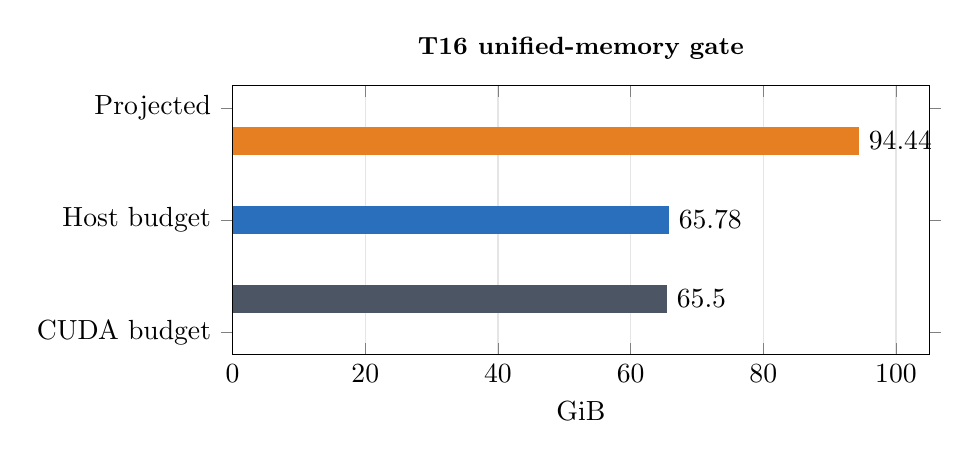
\begin{tikzpicture}
\begin{axis}[
  width=0.86\linewidth,height=5.0cm,
  xbar,xmin=0,xmax=105,
  xlabel={GiB},
  symbolic y coords={CUDA budget,Host budget,Projected},
  ytick={Projected,Host budget,CUDA budget},
  xmajorgrids=true,grid style={draw=gray!20},
  nodes near coords,nodes near coords align={horizontal},
  title={T16 unified-memory gate},
  title style={font=\small\bfseries},
]
\addplot[fill=reportorange,draw=none] coordinates {(94.435,Projected)};
\addplot[fill=reportblue,draw=none] coordinates {(65.784,Host budget)};
\addplot[fill=reportgray,draw=none] coordinates {(65.496,CUDA budget)};
\end{axis}
\end{tikzpicture}
}%
\end{minipage}\hfill
\begin{minipage}{0.44\textwidth}
\centering
\resizebox{\linewidth}{!}{%
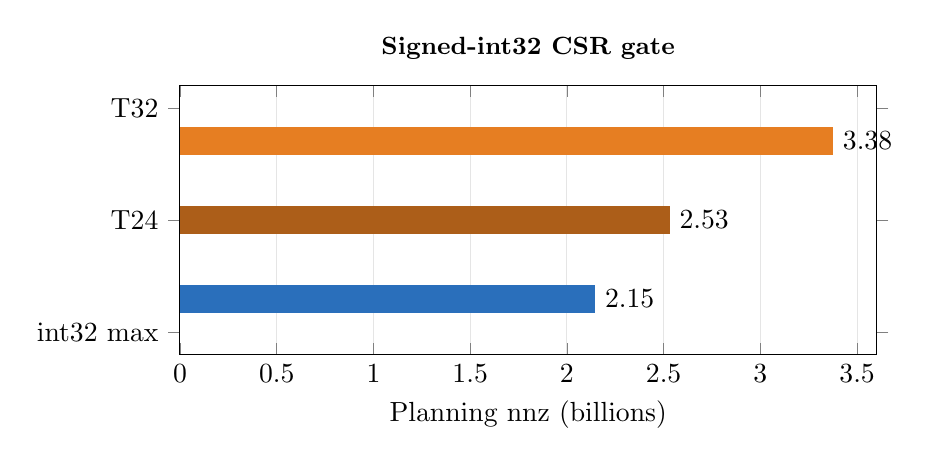
\begin{tikzpicture}
\begin{axis}[
  width=0.86\linewidth,height=5.0cm,
  xbar,xmin=0,xmax=3.6,
  xlabel={Planning nnz (billions)},
  symbolic y coords={int32 max,T24,T32},
  ytick={T32,T24,int32 max},
  xmajorgrids=true,grid style={draw=gray!20},
  nodes near coords,nodes near coords align={horizontal},
  title={Signed-int32 CSR gate},
  title style={font=\small\bfseries},
]
\addplot[fill=reportorange,draw=none] coordinates {(3.376,T32)};
\addplot[fill=reportorange!75!black,draw=none] coordinates {(2.532,T24)};
\addplot[fill=reportblue,draw=none] coordinates {(2.147,int32 max)};
\end{axis}
\end{tikzpicture}
}%
\end{minipage}
\caption{Preallocation safety boundaries for the final requested Stage 8 rows.
These are fail-closed resource outcomes, not runtime OOM crashes.}
\label{fig:resources}
\end{figure*}

The maximum cumulative process-lifetime host high-water mark was 95.375 GiB
at T6. It is not an isolated solve peak. CUDA snapshots likewise bracket
solves but do not expose a true per-solve GPU high-water mark through this
backend.

\section{Differences from the Paper}

\subsection{Matched structure}

The canonical signs, variables, constraint families, all 18 $(m,n)$ pairs,
paper update order, Halpern weights, tolerance, ten Ruiz passes,
Pock--Chambolle $\alpha=1$, initial $\sigma=1$, 100-iteration policy cadence,
CSR storage, and requested ALG2 path are reproduced. FP64 CPU/GPU trajectories
and accepted original-space numerical checks agree.

\subsection{Reconstructed or unavailable identity}

Renewable/storage placement, time profiles, reserves, ramps, device parameters,
costs, PTDF reference and sparsification, exact penalty/restart code, author
source, and timer boundary are unavailable. All 18 reconstructed nonzero counts
differ from Table II; observed differences range from approximately -8.14\%
to -36.66\%. The GB10 stack differs from the A100 environment.

\subsection{Retained manuscript ambiguities}

Equation (55) and Table II imply $m_1=T+N_{ESS}$, whereas Appendix A prose
implies $T(1+N_{ESS})$. The rank-one inverse sign is inconsistent with its
Schur complement. The objective-error denominator, precision, spectral
estimator, PTDF thresholding, source revisions, and exact timer boundary are
not fully specified. The security-constrained label lacks an explicit N-1
formulation.

\section{Final Reproduction Classification}

\begin{table*}[t]
\caption{Frozen A--E classification decision.}
\label{tab:classification}
\centering
\small
\begin{tabular}{@{}clp{0.72\textwidth}@{}}
\toprule
Code & Label & Decision \\
\midrule
A & Exact & Rejected: author instances, code, hardware, and exact outputs are unavailable. \\
B & Near-exact & Rejected: every sparse nnz differs and timing is not hardware-controlled. \\
C & Mathematical & Achieved but incomplete as the final label: the benchmark structure was also reconstructed and executed. \\
\textbf{D} & \textbf{Structural} & \textbf{Selected: mathematics, implementation, dimensions, public-network scaling, validation, and resource limits are reproduced with transparently reconstructed data.} \\
E & Partial & Rejected: the evidence exceeds an isolated component or incomplete prototype despite the honest Stage 8 failure. \\
\bottomrule
\end{tabular}
\end{table*}

Classification is an evidence boundary, not a stage-score average. Exact
instance identity is unavailable, but the work includes 18 symbolic rows, 11
allocated GPU-validated rows, 10 CPU-validated rows, full provenance,
independent checks, and fail-closed resource accounting. The defensible final
label is \classresult{}.

\section{Limitations and Next Research Step}

The dominant limitation is author-instance provenance, not tuning. Local
timings cannot isolate hardware, sparse support, runtime, algorithm, and timer
effects. Stage 8 does not fully validate T6 because CPU FP64 timed out. The
three final rows establish safe local resource limits but no solver timing.
Available memory APIs provide snapshots and cumulative host high-water marks,
not isolated peaks. The control policy is a sourced reconstruction. Finally,
this is base-case DCOPF, not N-1 security analysis.

The highest-value next step is author-instance reconciliation: obtain modified
case files, time series, placements, physical parameters, construction code,
precision, policy implementation, and timing rules. Exact $m$, $n$, and nnz
should first be matched on small rows, followed by objective/KKT fingerprints
and an equivalent A100 timing boundary. If author artifacts remain unavailable,
a verified 64-bit or partitioned sparse representation and lower-peak assembly
would form a new scalability study, not a revision of the present result.
Stage 10 remains locked.

\section{Conclusion}

The project rebuilt and checked the paper's route from canonical DCOPF to a
resident FP64 GPU solver. It identified a material algebraic sign error,
separated stopping from full KKT validation, demonstrated CPU/GPU trajectory
parity, and preserved every large-run outcome without weakening a gate. Public
reconstructions scale to hundreds of millions of sparse nonzeros but are not
the authors' instances. The large campaign contains a genuine CPU timeout and
two distinct preallocation ceilings. The scientifically defensible conclusion
is \classresult{}: stronger than a partial port and narrower than a near-exact
replication.

\appendices

\section{Full Evidence Ledger}

The independent checker totals are: Stage 0, 10/10; Stage 1, 6/6; Stage 2,
9/9; Stage 3, 12/12; Stage 4, 20/20; Stage 5, 23/23; Stage 6, 21/21; Stage 7,
19/19; Stage 8 strict protocol, 12/12; and Stage 8 GPU-only continuation,
13/13. Exact paths and hashes are in
\pathcode{results/stage_9_result_index.json}. Checker totals establish
evidence integrity but do not replace stage decisions.

\section{Structural Reconciliation}

The complete 18-row ledger is
\pathcode{results/tables/stage_9_structural_reconciliation.csv}. Every row has
matching published/reproduced $m$ and $n$; zero rows have matching nnz; and
zero rows are paper-time-comparable. Unallocated large-row counts are symbolic
or count-only evidence, not materialized LPs.

\section{Missing Source Information}

Exact numerical reproduction would require:
\begin{itemize}
  \item exact base-case files, versions, and hashes;
  \item renewable and storage bus locations;
  \item load/renewable/reserve time series, ramps, storage parameters, and
  cost modifications;
  \item PTDF slack/reference choice, transformer/island handling, and sparse
  zero threshold;
  \item exact adaptive-penalty, restart, spectral-estimation, safety, and
  precision rules;
  \item author CUDA/source revisions and build flags; and
  \item exact timer inclusion boundary, repeat protocol, and variance data.
\end{itemize}

\section{Reproducibility Checklist}

The durable checklist is \pathcode{docs/reproducibility_checklist.md}. It
covers source identity, mathematical derivation, physical validation,
CPU/GPU parity, benchmark protocol, report QA, and the Stage 10 lock.

\section{Regeneration and Test Commands}

Run from the repository root:
\begin{lstlisting}
python scripts/generate_stage_9_artifacts.py
python scripts/generate_stage_9_artifacts.py --check
python scripts/check_stage_9.py --output results/raw/stage_9/stage_9_checks.json
python -m pytest -q
python -m ruff check .
python -m ruff format --check .
cd dashboard
npm test
npm run lint
cd ..
\end{lstlisting}
The complete per-table, PDF-rendering, and earlier-checker command inventory is
\pathcode{docs/regeneration_commands.md}. Accepted Stage 7--8 benchmark
evidence is immutable; rebuilding this report does not rerun benchmark
allocations.

\section{Machine-Readable Result Index}

\pathcode{results/stage_9_result_index.json} records paper identity, final
classification, stage/checker decisions, Stage 8 failure and continuation
semantics, coverage totals, environment, frozen gates, evidence hashes, table
and figure hashes, and the explicit Stage 10 lock.

\section{Final Git-State Boundary}

A commit cannot embed its own identifier without changing that identifier.
The report records the tested source HEAD and verifies the final repository
externally:
\begin{lstlisting}
git diff --check
git status --short
git rev-parse HEAD
git log -1 --format=fuller
\end{lstlisting}
The final handoff requires no output from \texttt{git status --short}; the
actual final commit and push result accompany the completion notice.

\begin{thebibliography}{9}

\bibitem{wang2026}
Q. Wang, G. Zhang, Y. Yang, C. Ren, W. Wu, X. Zhao, M. Skoglund, and D. Sun,
``An efficient GPU-based Halpern accelerating algorithm for large-scale DC
optimal power flow,'' \emph{IEEE Trans. Power Syst.}, vol. 41, no. 3,
pp. 2187--2204, May 2026, doi: 10.1109/TPWRS.2025.3635652.

\bibitem{matpower}
R. D. Zimmerman, C. E. Murillo-Sanchez, and R. J. Thomas, ``MATPOWER:
Steady-state operations, planning, and analysis tools for power systems
research and education,'' \emph{IEEE Trans. Power Syst.}, vol. 26, no. 1,
pp. 12--19, Feb. 2011.

\bibitem{highs}
Q. Huangfu and J. A. J. Hall, ``Parallelizing the dual revised simplex
method,'' \emph{Math. Program. Comput.}, vol. 10, pp. 119--142, 2018.

\bibitem{pockchambolle}
T. Pock and A. Chambolle, ``Diagonal preconditioning for first order primal-dual
algorithms in convex optimization,'' in \emph{Proc. IEEE ICCV}, 2011,
pp. 1762--1769.

\end{thebibliography}

\end{document}
